\pgfplotsset{
	axis background/.style={fill=white},
	tick style=black,
	tick label style=black,
	grid=both,
	xtick pos=left,
	ytick pos=left,
	tick style={
		major grid style={style=white,line width=1pt},minor grid style=white,
		tick align=outside,
	},
	minor tick num=4,
}

\begin{figure}[!h]
\centering
    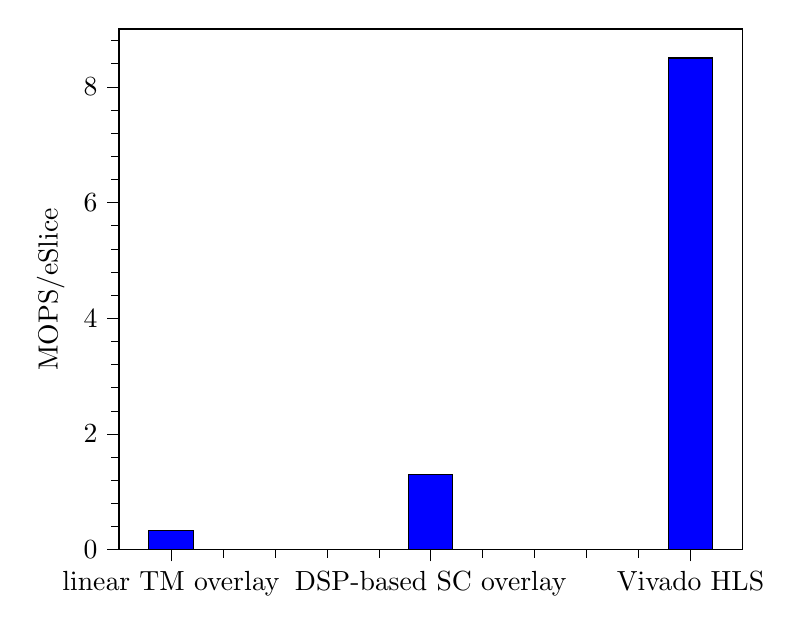
\begin{tikzpicture}
    \begin{axis}[
    ymin=0,ymax=9,
    width=9.5cm,
    bar width=16pt,
    ylabel=MOPS/eSlice,
    symbolic x coords={linear TM overlay, DSP-based SC overlay, Vivado HLS},
    xtick=data
    ]
    \addplot[ybar,fill=blue] coordinates {
    	(linear TM overlay,   0.33)
    	(DSP-based SC overlay,  1.3)
    	(Vivado HLS,   8.5)
    };      
    \end{axis}
    \end{tikzpicture}
\caption{Average compute efficiency in MOPS/eSlice.}
\label{compute_efficiency}
\end{figure}
